\section{Using Kathará. Practical case study}
\label{sec:katharapracticalcasestudy}

For the practical case study of Kathará, we followed the same approach than for GNS3's, used the same lab handouts from APRC as reference, but implemented in Kathará's different paradigm.
Refer to section~\ref{sec:gns3practicalcasestudy} for an overview of the labs and their topics.

\subsection{Setting topologies in Kathará}

As mentioned earlier in this chapter, Kathará doesn't offer a graphical interface to draw topologies, and nodes added and removed, started and stopped, and text-based consoles to them are created via a set shell commands.

We mentioned as well that, in Kathará, there aren't end-to-end links as such, like there are on GNS3.
Instead, Kathará has collision domains, which are Ethernet media, shared by whichever interfaces are attached to them, and all hosts connected through a collision domain can have packets sent back and forth among each other.
For instance, each IP-prefix corresponding to a logical LAN, connected to a layer-3 router, can have all its hosts attached to the same collision domain.

In spite of the aforementioned, to be coherent with what was done in the GNS3 case-study and to be able to compare both frameworks more fairly---and because it is a condition to perform the switching assignment, in lab handout~2---it was decided that we would always use point-to-point links, which in practice means creating as many collision domains as there are links, and attaching each corresponding pair of interfaces in the nodes to every correct one. % TODO este point-to-point está certo?

% Figure fig:kathara-annotated-lab3-topology
\begin{figure}
  \centering
  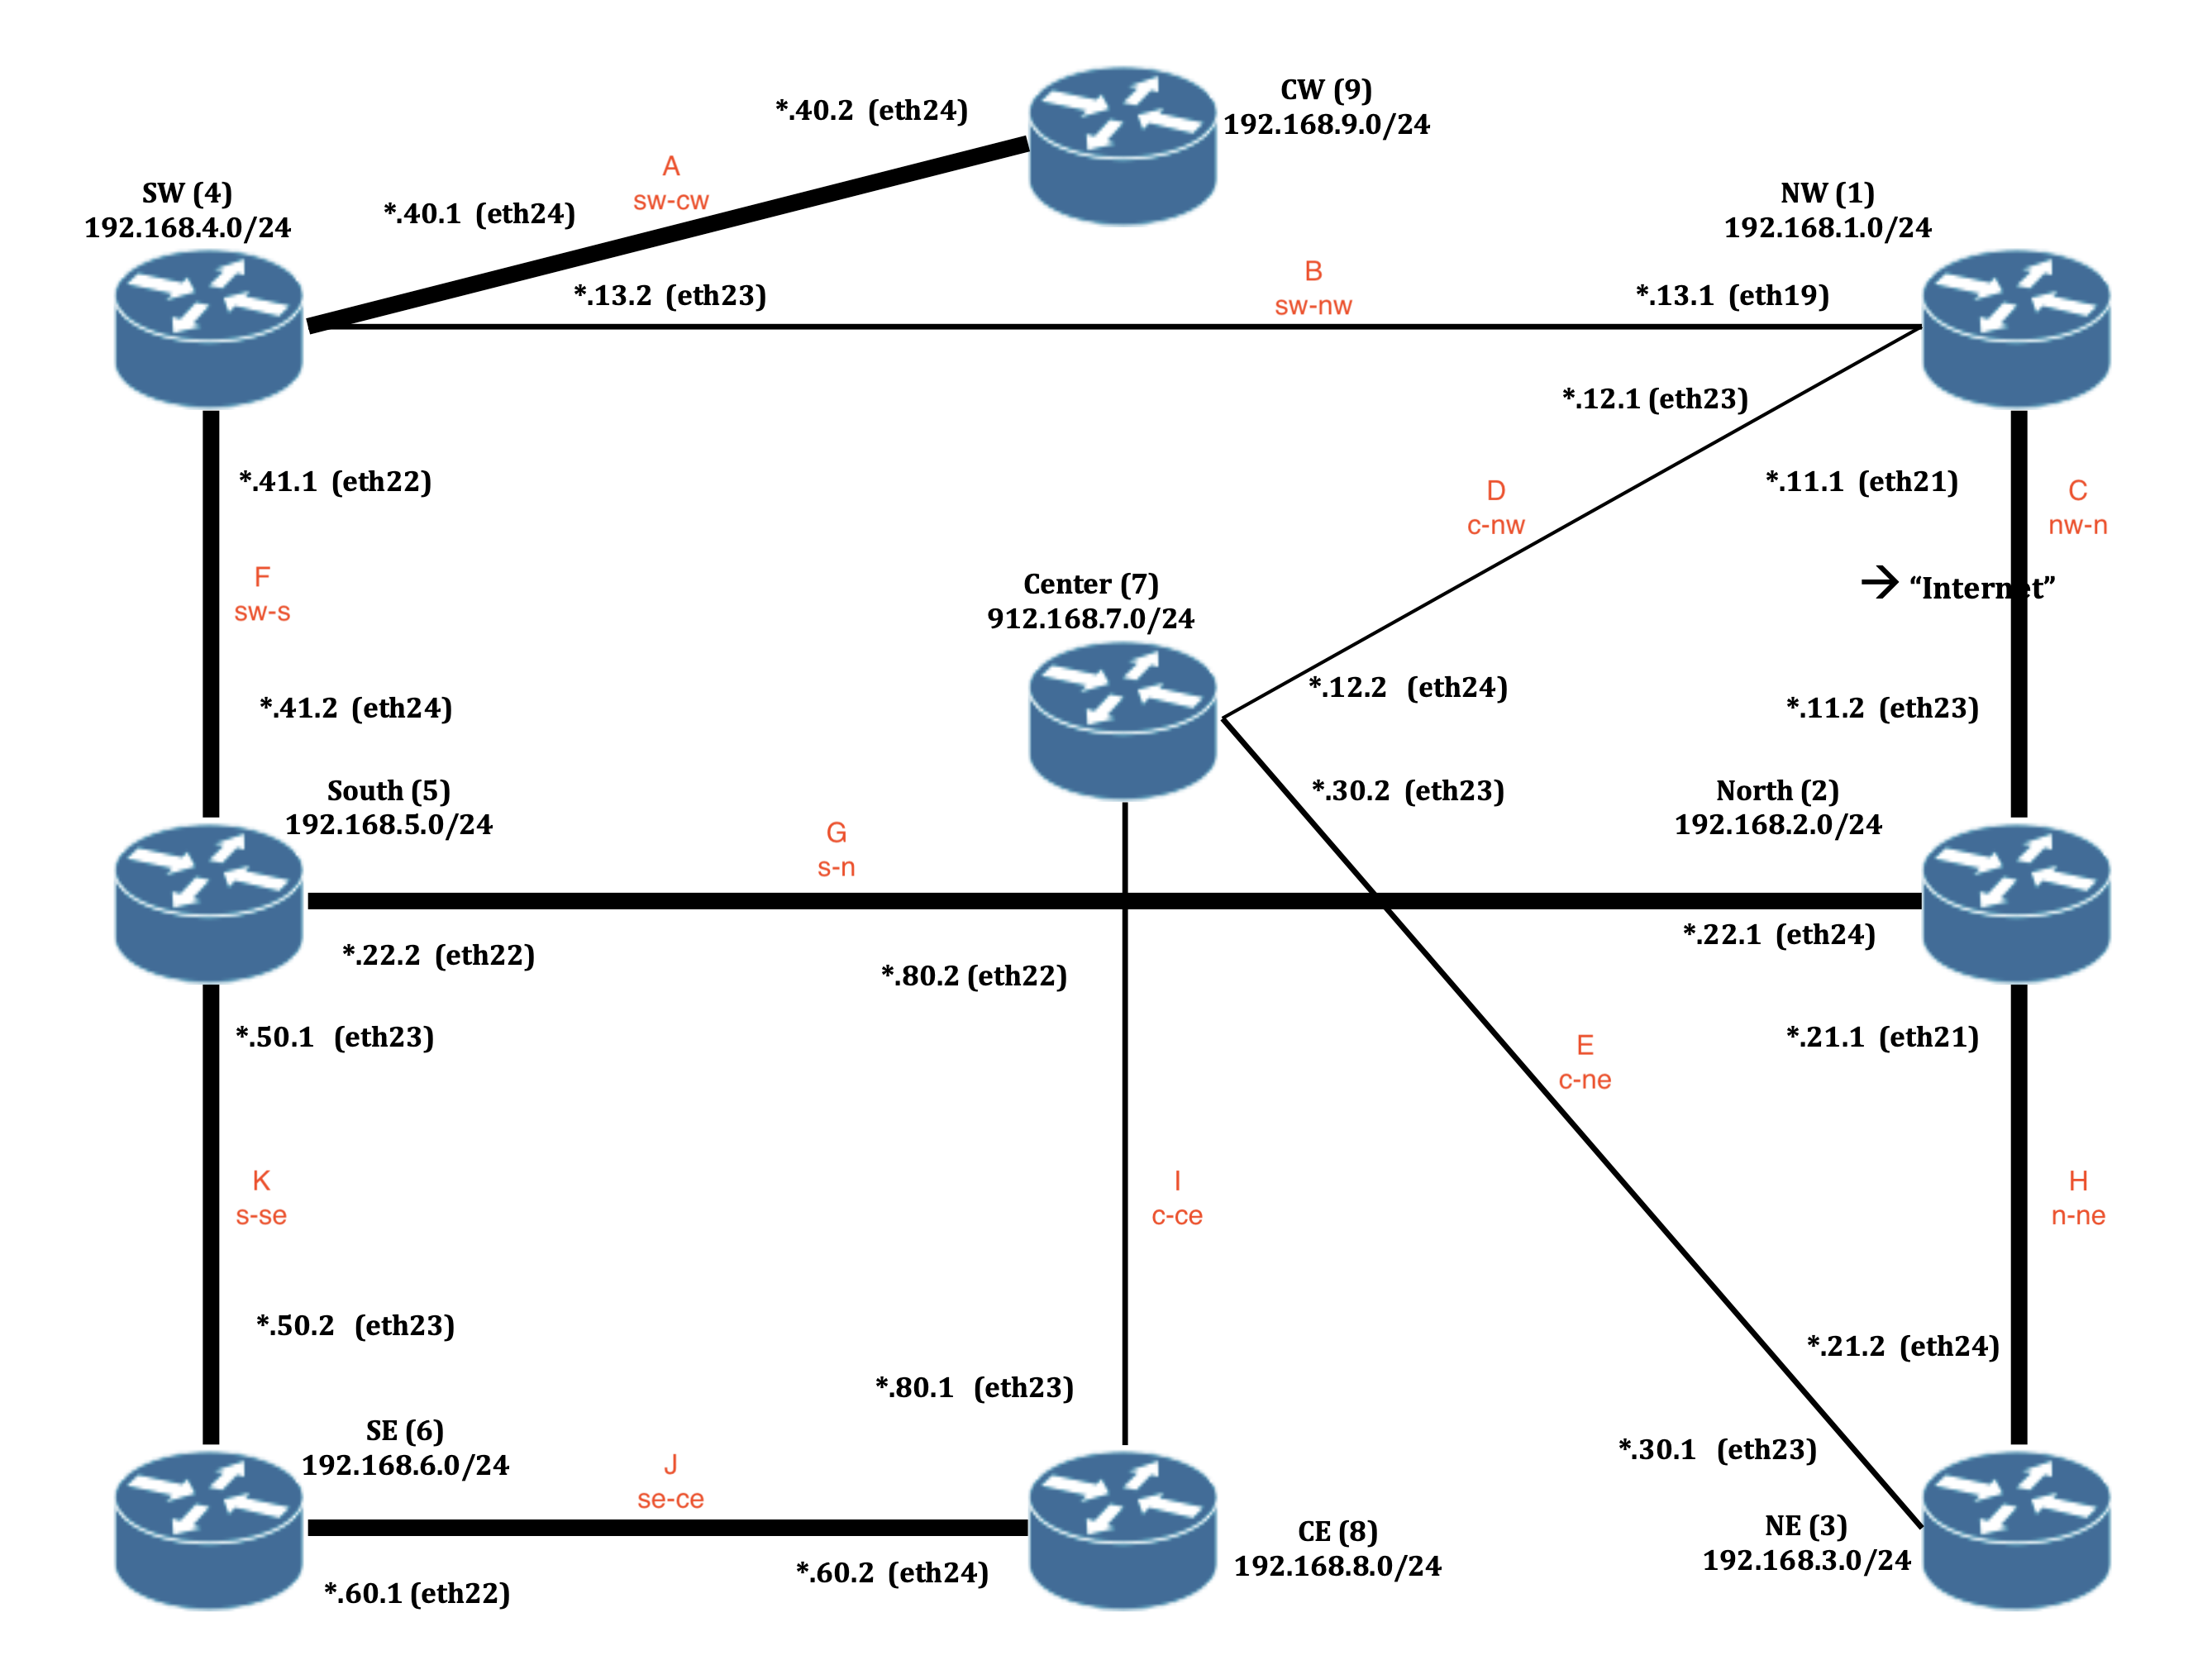
\includegraphics[width=\textwidth]{kathara-annotated-lab3-topology}
  \caption{Section of ``lab-assignment3'' showing the topology, with every collision domain annotated}
  \label{fig:kathara-annotated-lab3-topology}
\end{figure}


To facilitate this process, the graphical representation of the topology as given in the course's handout PDF was annotated with the letters that are becoming each collision domain, as figure~\ref{fig:kathara-annotated-lab3-topology} depicts. % TODO fazer versão vectorial desta figura
Then, writing Kathará's \texttt{lab.conf} and making sure that it is correct becomes much easier.

\subsection{Switching exercises}

The switching lab was set up using a similar methodology than the one described just before for lab~3---i.e. the topology was graphically annotated to define the collision domains among the several interfaces.

Then, using Kathará's convention to ``pass-on'' configuration directories to each container, we defined the startup file (that is executed by its respective container when it ``boots up'') to setup a bridge virtual interface, according to the Linux bridge documentation and online resources~\cite{brctlman,howtobridgelinux}.

For the switching exercises, we found out that there is some kind of limitation, either in Docker itself, in Docker's chosen intercontainer networking strategy, or in Kathará's implementation.
The containers (lightweight virtual Linux hosts), equipped with multiple NICs that perform each switch, are not capable of successfully performing the Spanning Tree Protocol, which is demanding for a topology with a loop, witch the lab's deliberately has.  % TODO acronym in NIC

% end of section katharapracticalcasestudy
